\documentclass[a4paper,11pt]{article}

\usepackage[portuguese]{babel}
\usepackage[utf8]{inputenc}
\usepackage{amsmath}
\usepackage{graphicx}
\usepackage{hyperref}
\usepackage{float}
\usepackage{subfig}
\usepackage{fixltx2e}
\usepackage[bottom]{footmisc}
\usepackage{listings}
\usepackage{xargs}                      % Use more than one optional parameter in a new commands
\usepackage[pdftex,dvipsnames]{xcolor}  % Coloured text etc.
\usepackage[colorinlistoftodos,prependcaption,textsize=tiny]{todonotes}
\newcommandx{\unsure}[2][1=]{\todo[linecolor=red,backgroundcolor=red!25,bordercolor=red,#1]{#2}}
\newcommandx{\change}[2][1=]{\todo[linecolor=blue,backgroundcolor=blue!25,bordercolor=blue,#1]{#2}}
\newcommandx{\info}[2][1=]{\todo[linecolor=OliveGreen,backgroundcolor=OliveGreen!25,bordercolor=OliveGreen,#1]{#2}}
\newcommandx{\improvement}[2][1=]{\todo[linecolor=Plum,backgroundcolor=Plum!25,bordercolor=Plum,#1]{#2}}
\newcommandx{\thiswillnotshow}[2][1=]{\todo[disable,#1]{#2}}
\usepackage[font=footnotesize]{caption}
\usepackage[hypcap]{caption}
\usepackage[top=2.5cm, bottom=2.5cm, left=2.5cm, right=2.5cm]{geometry}
\usepackage{enumerate}
\usepackage[siunitx,american]{circuitikz}

\setcounter{tocdepth}{3}
\setcounter{secnumdepth}{4}

\numberwithin{equation}{section}
\addto\captionsportuguese{\renewcommand{\contentsname}{Índice}}

\linespread{1.3}
\usepackage{indentfirst}

\begin{document}
\begin{titlepage}
\begin{center}

\hfill \break
\hfill \break


\includegraphics[width=0.3\textwidth]{img/logo}~\\[1cm] 

\textsc{\LARGE Instituto Superior Técnico}\\[0.25cm]
\textsc{\Large Mestrado Integrado em Engenharia Electrotécnica e de Computadores}\\[1.8cm]
\textsc{\huge Electrónica de Potência}\\[0.25cm]

\vspace{6mm}

{\huge \bfseries Conversor CA/CC Monofásico \linebreak Comandado de Onda Completa \\[0.7cm]}
{\bfseries Rectificador de onda completa totalmente comandado e semi-comandado \\[1cm]}

\begin{tabular}{ l l }
	João Bernardo Sequeira de Sá & \hspace{2mm} n.º 68254 \\
	Maria Margarida Dias dos Reis & \hspace{2mm} n.º 73099 \\
	Rafael Augusto Maleno Charrama Gonçalves & \hspace{2mm} n.º 73786 \\
	Nuno Miguel Rodrigues Machado & \hspace{2mm} n.º 74236
\end{tabular}

\vspace{7mm}

Turno de Segunda-feira das 17h00 - 20h00

\vfill

{\large Lisboa,  de Novembro de 2015} 
	
\end{center}
\end{titlepage}
	
\tableofcontents
\pagebreak

\section{Introdução}

Este trabalho laboratorial é uma continuação do trabalho 2A em que se estudou o conversor CA/CC (retificador) de meia onda comandado e semi-comandado monofásico. Desta vez o objetivo é compreender o funcionamento do retificador monofásico comandado de onda completa.

Este trabalho está separado em duas partes; na primeira estuda-se o funcionamento do conversor totalmente comandado e na segunda o semi-comandado.

Aquilo que distingue o retificador de onda completa do de meia onda é a presença de 4 tiristores, tal como pode ser observado na \autoref{fig:circuit_1}, em oposição a apenas 1 tiristor como se tinha no retificador de meia onda.


\begin{figure}[h]
	\centering
	%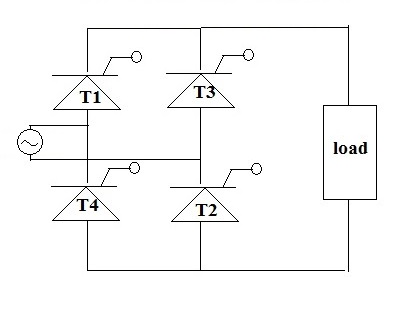
\includegraphics[keepaspectratio=true, scale=0.8]{img/circuito}
	\begin{tikzpicture}
	\draw
		(0,0) node[] (origin) {} to[sV] ++(0,2) node[] (source) {}
		(origin) to[short,-*] ++ (5,0) to[short] ++ (0,2) to[Ty,-*] ++ (0,2) to[short] ++ (2,0) to[generic,l=Carga] ++ (0,-6) to[short] ++ (-2,0) node[] (bottomty) {} to[short] ++(-2,0) to[Ty] ++ (0,2) to[short,-*] ++ (0,2) node[] (topty) {} to[short] (source)
		(bottomty) to[Ty,*-*] ++ (0,2)
		(topty) to[Ty] ++(0,2) to[short] ++ (2,0)
		;
	\end{tikzpicture}
	\caption{Esquema do retificador de onda completa monofásico comandado.}
	\label{fig:circuit_1}
	\vspace{-0.8em}
\end{figure}

O funcionamento desta topologia depende de qual o par de tiristores que está a conduzir a uma dada altura. Fazendo uso da nomenclatura da \autoref{fig:circuit_1} observa-se que T1 e T2 podem ser disparados durante a alternância positiva da tensão de entrada, sendo que T4 e T3 podem ser disparados durante a alternância negativa \cite{Silva}. Para o primeiro caso tem-se que o ângulo de disparo, $\alpha$, pode variar entre $0$ e $\pi$ onde para o segundo caso se faz uso de $\alpha + \pi$. Tal como já foi visto no trabalho anterior a altura em que um tiristor entra ao corte depende do momento em que a corrente aos terminais deste passa por zero, pelo que o funcionamento para uma carga puramente resistiva difere do de uma carga indutiva.

Espera-se assim que as formas de onda para a tensão e corrente numa carga indutiva seja tal como se vê na \autoref{fig:andamento}.

\begin{figure}[h]
	\centering
	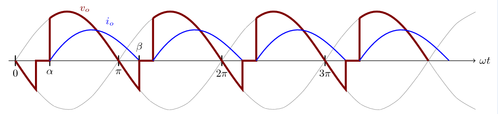
\includegraphics[keepaspectratio=true, scale=0.8]{img/andamento}
	\caption{Formas de onda para carga indutiva.}
	\label{fig:andamento}
	\vspace{-0.8em}
\end{figure}

O resultado é que, ao contrário do retificador de meia onda, tanto para a alternância positiva da tensão de entrada, como para a negativa, se irá ter corrente na carga; obtém-se um comportamento desta corrente muito mais próximo do continuo e um conteúdo harmónico substancialmente inferior. Observa-se também que devido a isto, o valor médio da corrente na entrada será zero.

Para a segunda parte do trabalho tem-se um retificador semi-comandado, onde se substitui dois do retificadores por dois díodos. Isto pode ser feito caso a carga não exija inversão da tensão aos seus terminais, sendo neste caso imposição da topologia que a tensão de saída tenha sempre o mesmo sinal, devido à presença dos díodos.


\section{Condução do Trabalho}

\subsection{Retificador de onda completa totalmente comandado}


\subsubsection{Carga resistiva pura (R)}


\paragraph{Formas de onda da tensão e corrente na entrada} \mbox{}\

\begin{figure}[H]
	\centering
	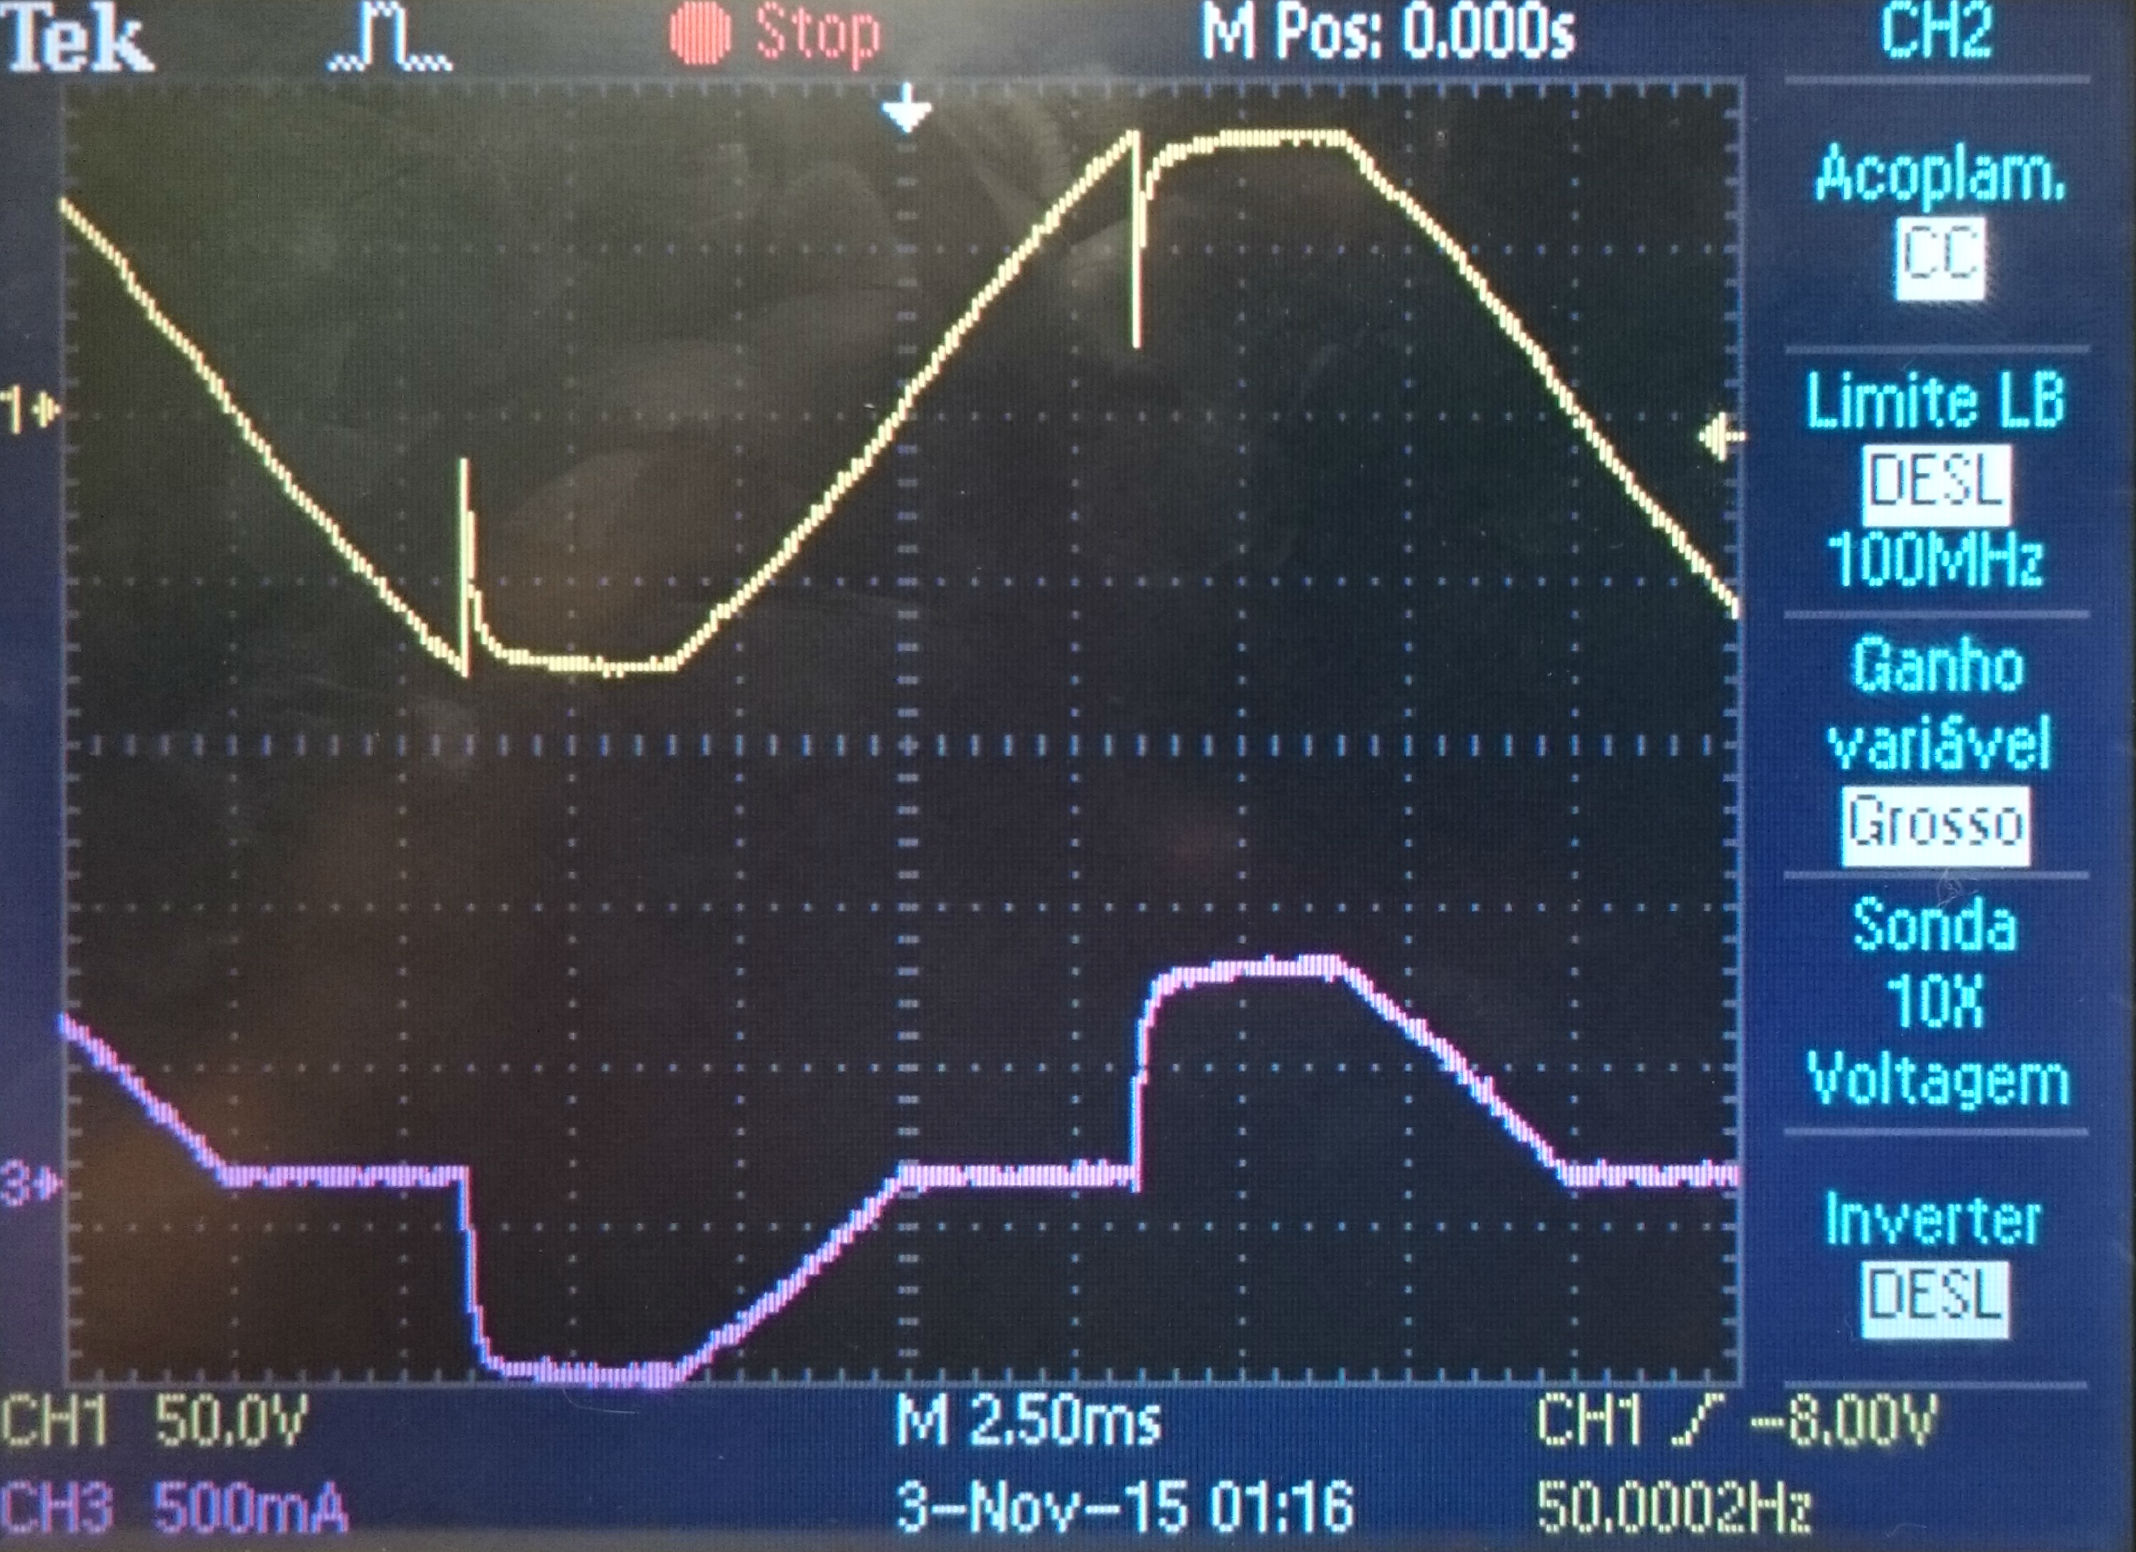
\includegraphics[keepaspectratio=true, scale=0.12]{img/DSC_0181}
	\caption{Tensão (a amarelo) e corrente (a rosa) na entrada.}
	\label{fig:tcentrada}
	\vspace{-0.8em}
\end{figure}

\paragraph{Formas de onda da tensão e corrente na carga} \mbox{}\


\begin{figure}[H]
	\centering
	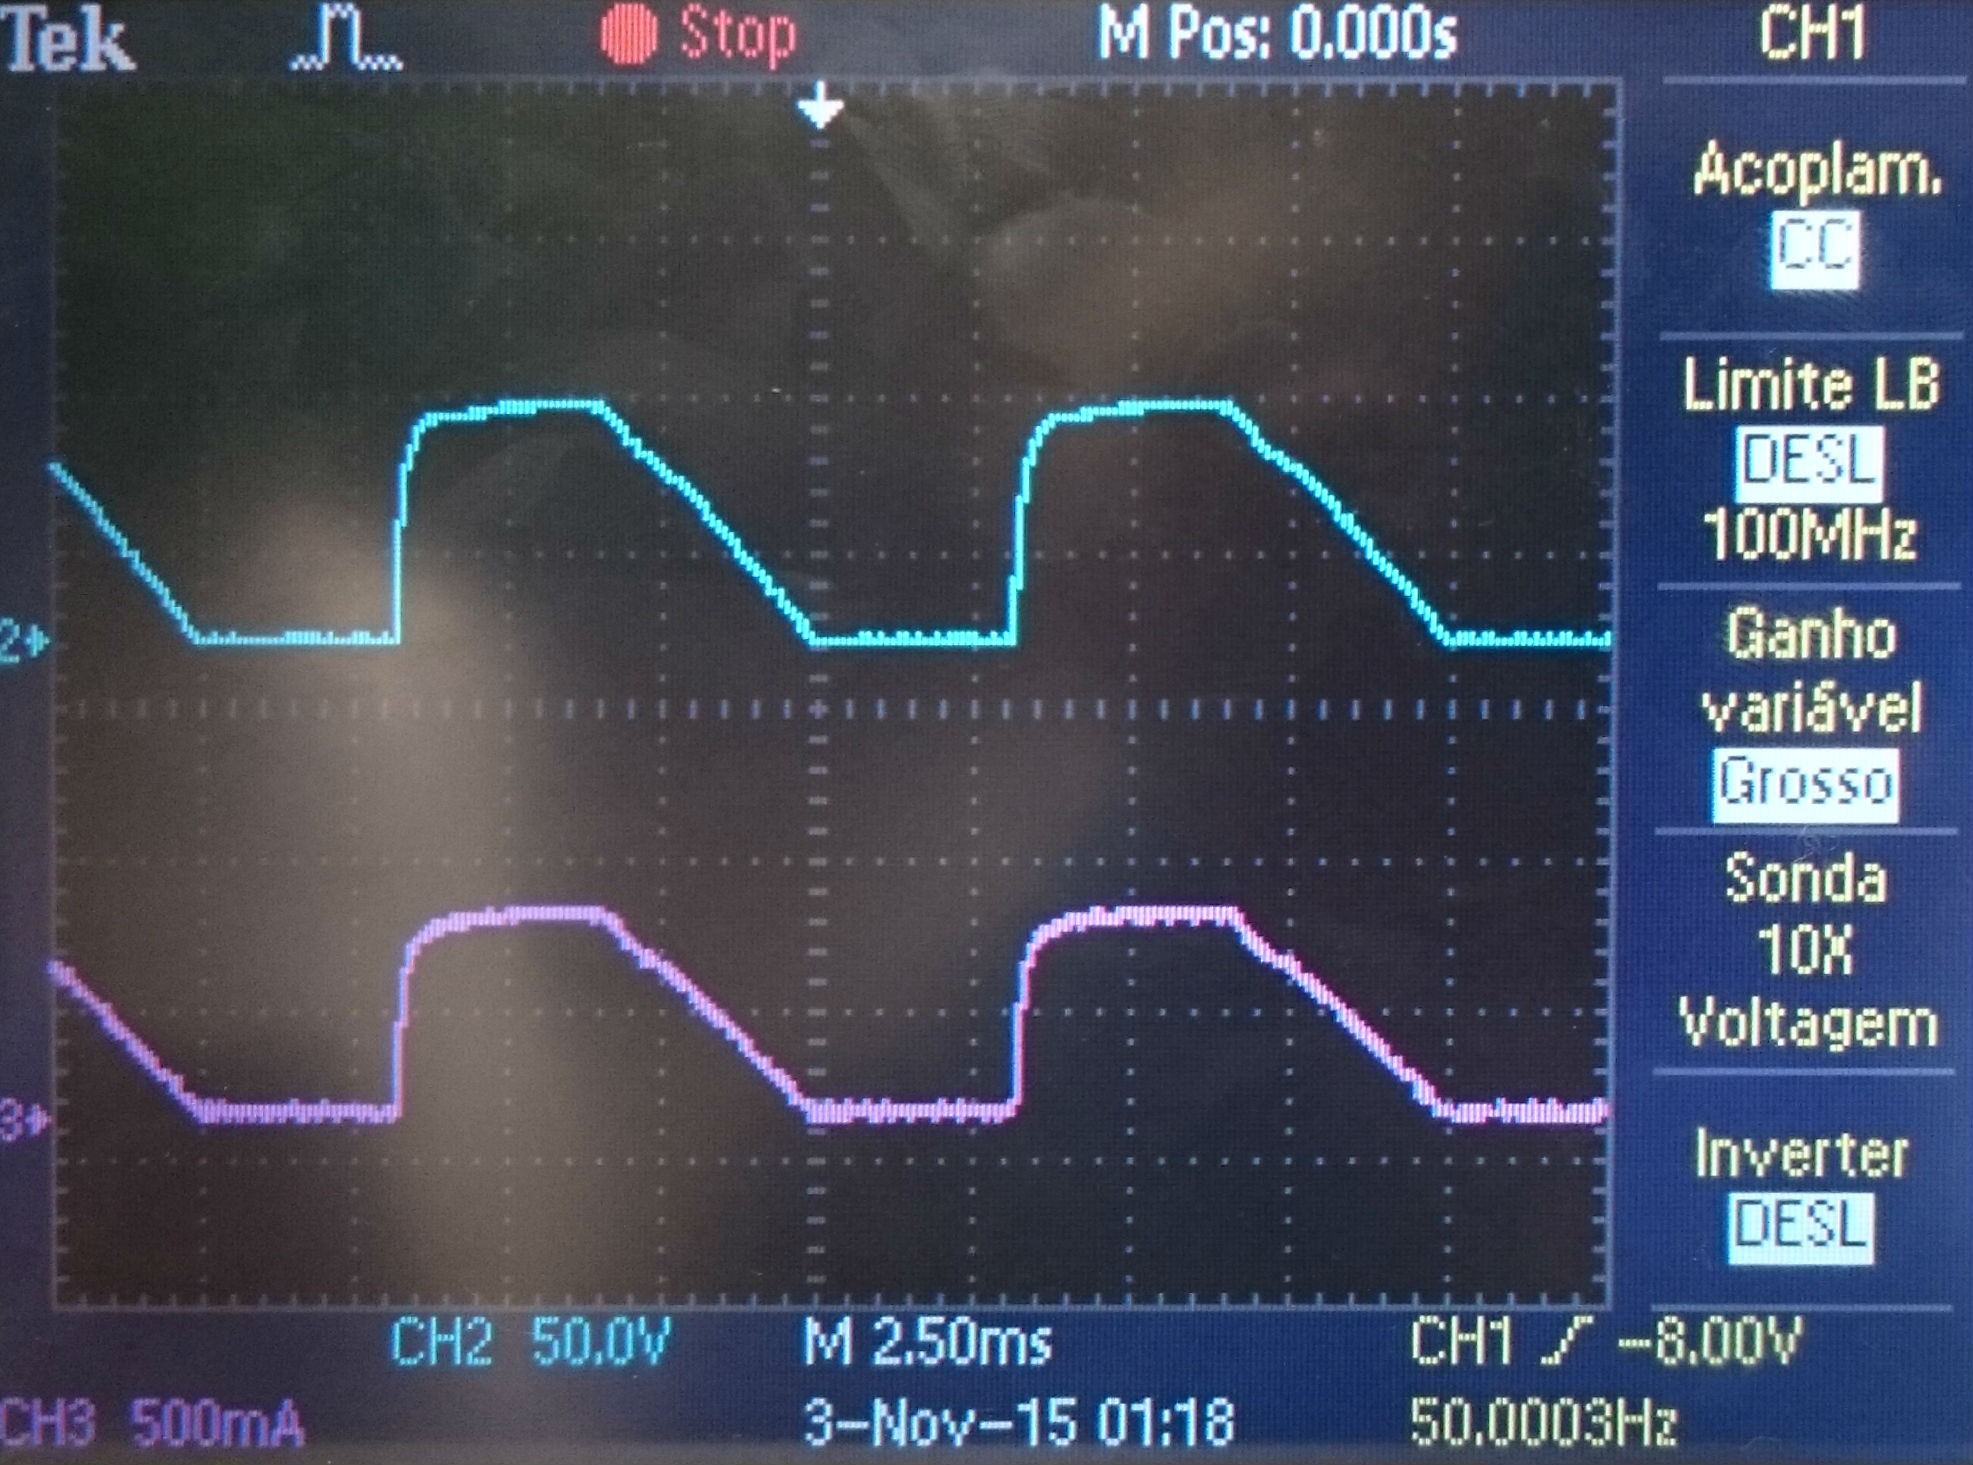
\includegraphics[keepaspectratio=true, scale=0.13]{img/DSC_0182}
	\caption{Tensão (a azul) e corrente (a rosa) na carga.}
	\label{fig:tccarga}
	\vspace{-0.8em}
\end{figure}

\paragraph{Formas de onda da tensão e corrente no tiristor} \mbox{}\

\begin{figure}[H]
	\centering
	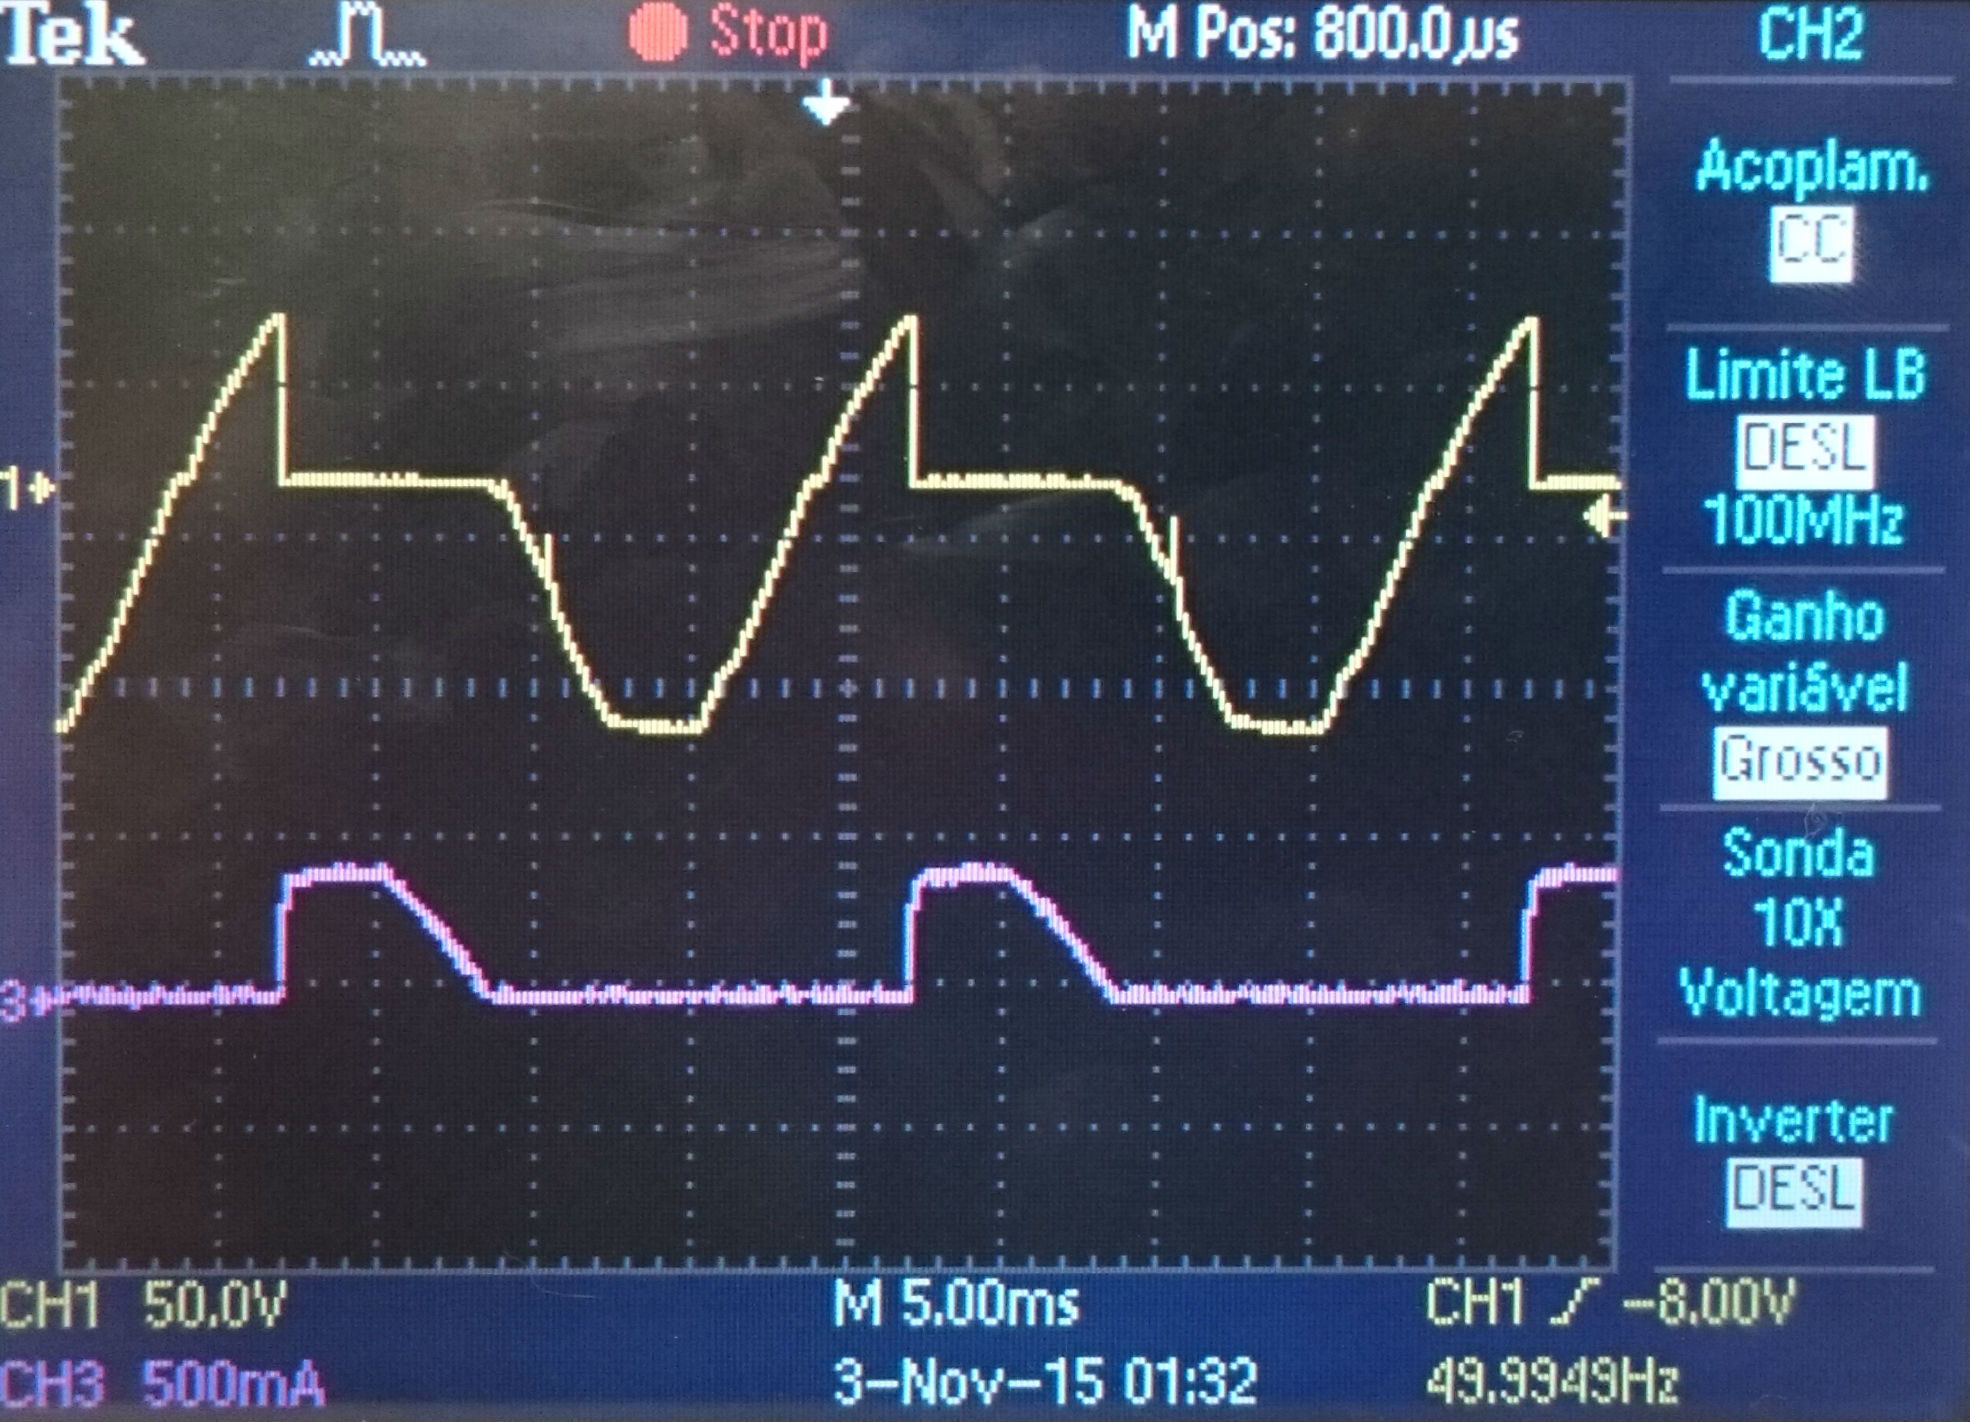
\includegraphics[keepaspectratio=true, scale=0.13]{img/DSC_0183}
	\caption{Tensão (a amarelo) e corrente (a rosa) no tiristor.}
	\label{fig:tctiristor}
	\vspace{-0.8em}
\end{figure}

\paragraph{Característica de comando do conversor} \mbox{}\

\subsubsection{Carga indutiva RL}

\paragraph{Formas de onda da tensão e corrente na carga para funcionamento lacunar} \mbox{}\

\begin{figure}[H]
	\centering
	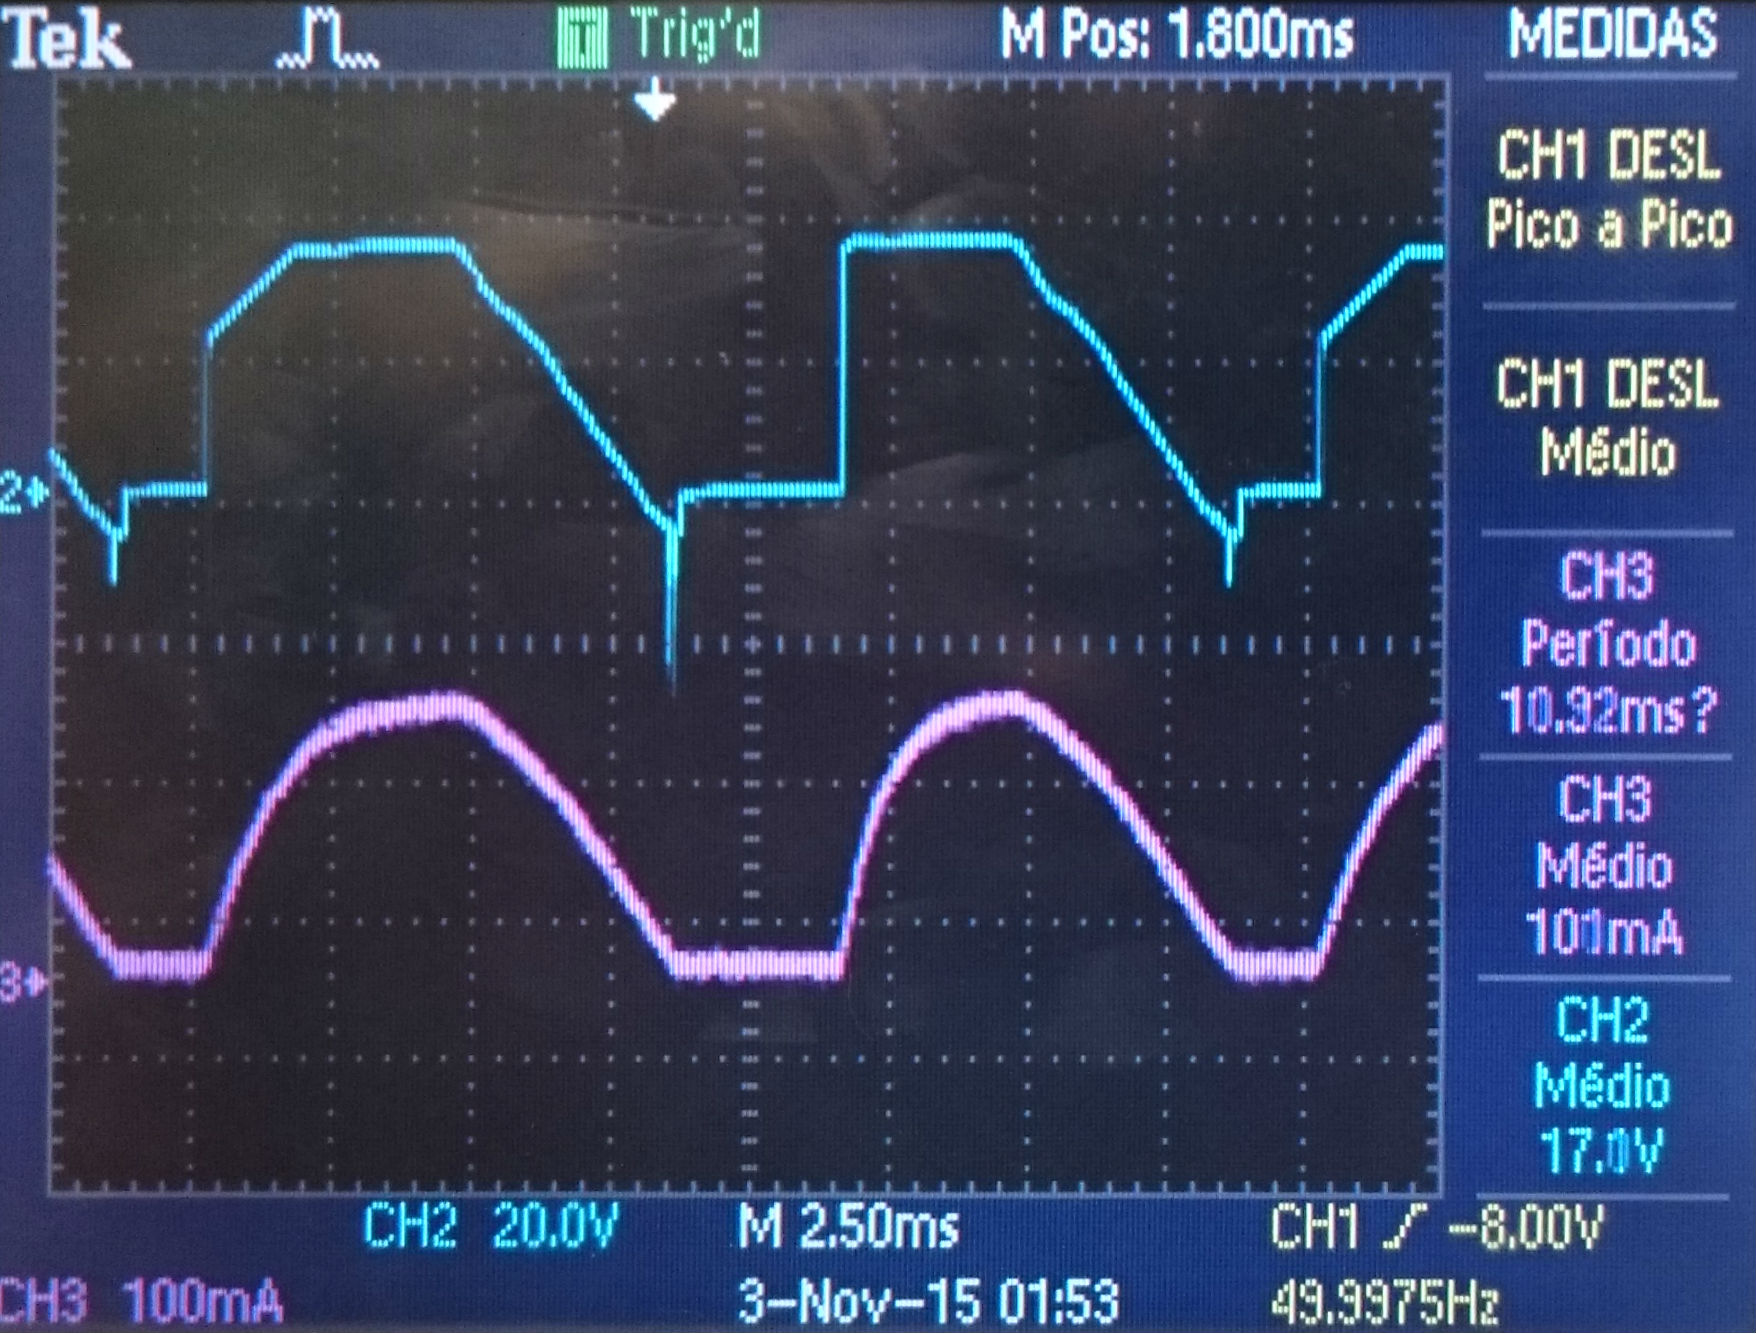
\includegraphics[keepaspectratio=true, scale=0.15]{img/DSC_0184}
	\caption{Tensão (a azul) e corrente (a rosa) na carga.}
	\label{fig:tcentradalacuna}
	\vspace{-0.8em}
\end{figure}

\todo{dizer porque razão a tensão na carga é negativa por algum tempo}

\todo{tensão medida na carga}

\paragraph{Formas de onda da tensão e corrente no tiristor} \mbox{}\

\begin{figure}[H]
	\centering
	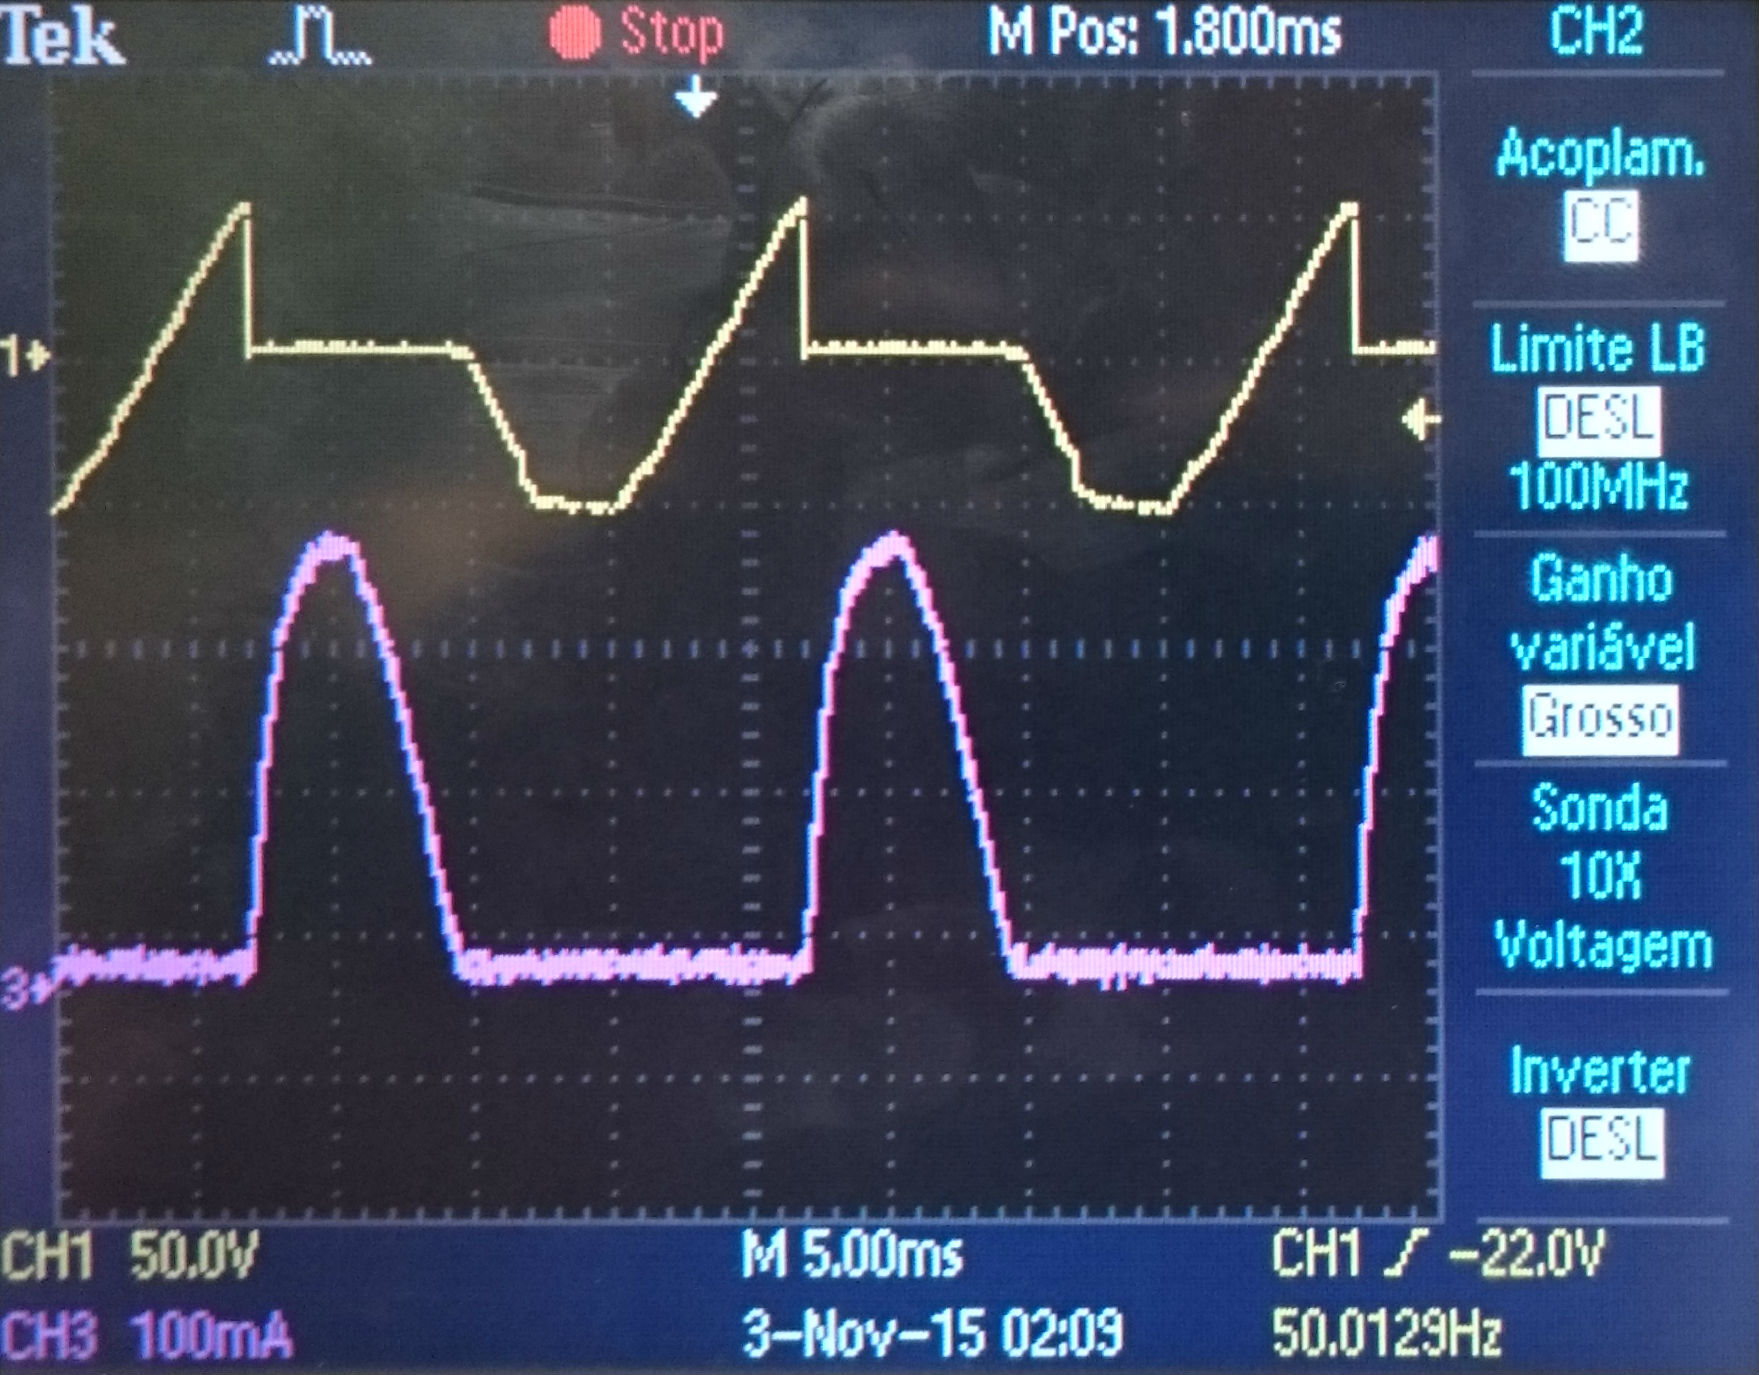
\includegraphics[keepaspectratio=true, scale=0.15]{img/DSC_0185}
	\caption{Tensão (a amarelo) e corrente (a rosa) no tiristor.}
	\label{fig:tctiristorlacuna}
	\vspace{-0.8em}
\end{figure}

\paragraph{Formas de onda da tensão e corrente para funcionamento não lacunar} \mbox{}\

\paragraph{Característica de comando do conversor} \mbox{}\

\subsection{Retificador de onda completa semi-comandado}

\subsubsection{Carga indutiva RL}

\paragraph{Formas de onda da tensão e corrente na entrada} \mbox{}\

\begin{figure}[H]
	\centering
	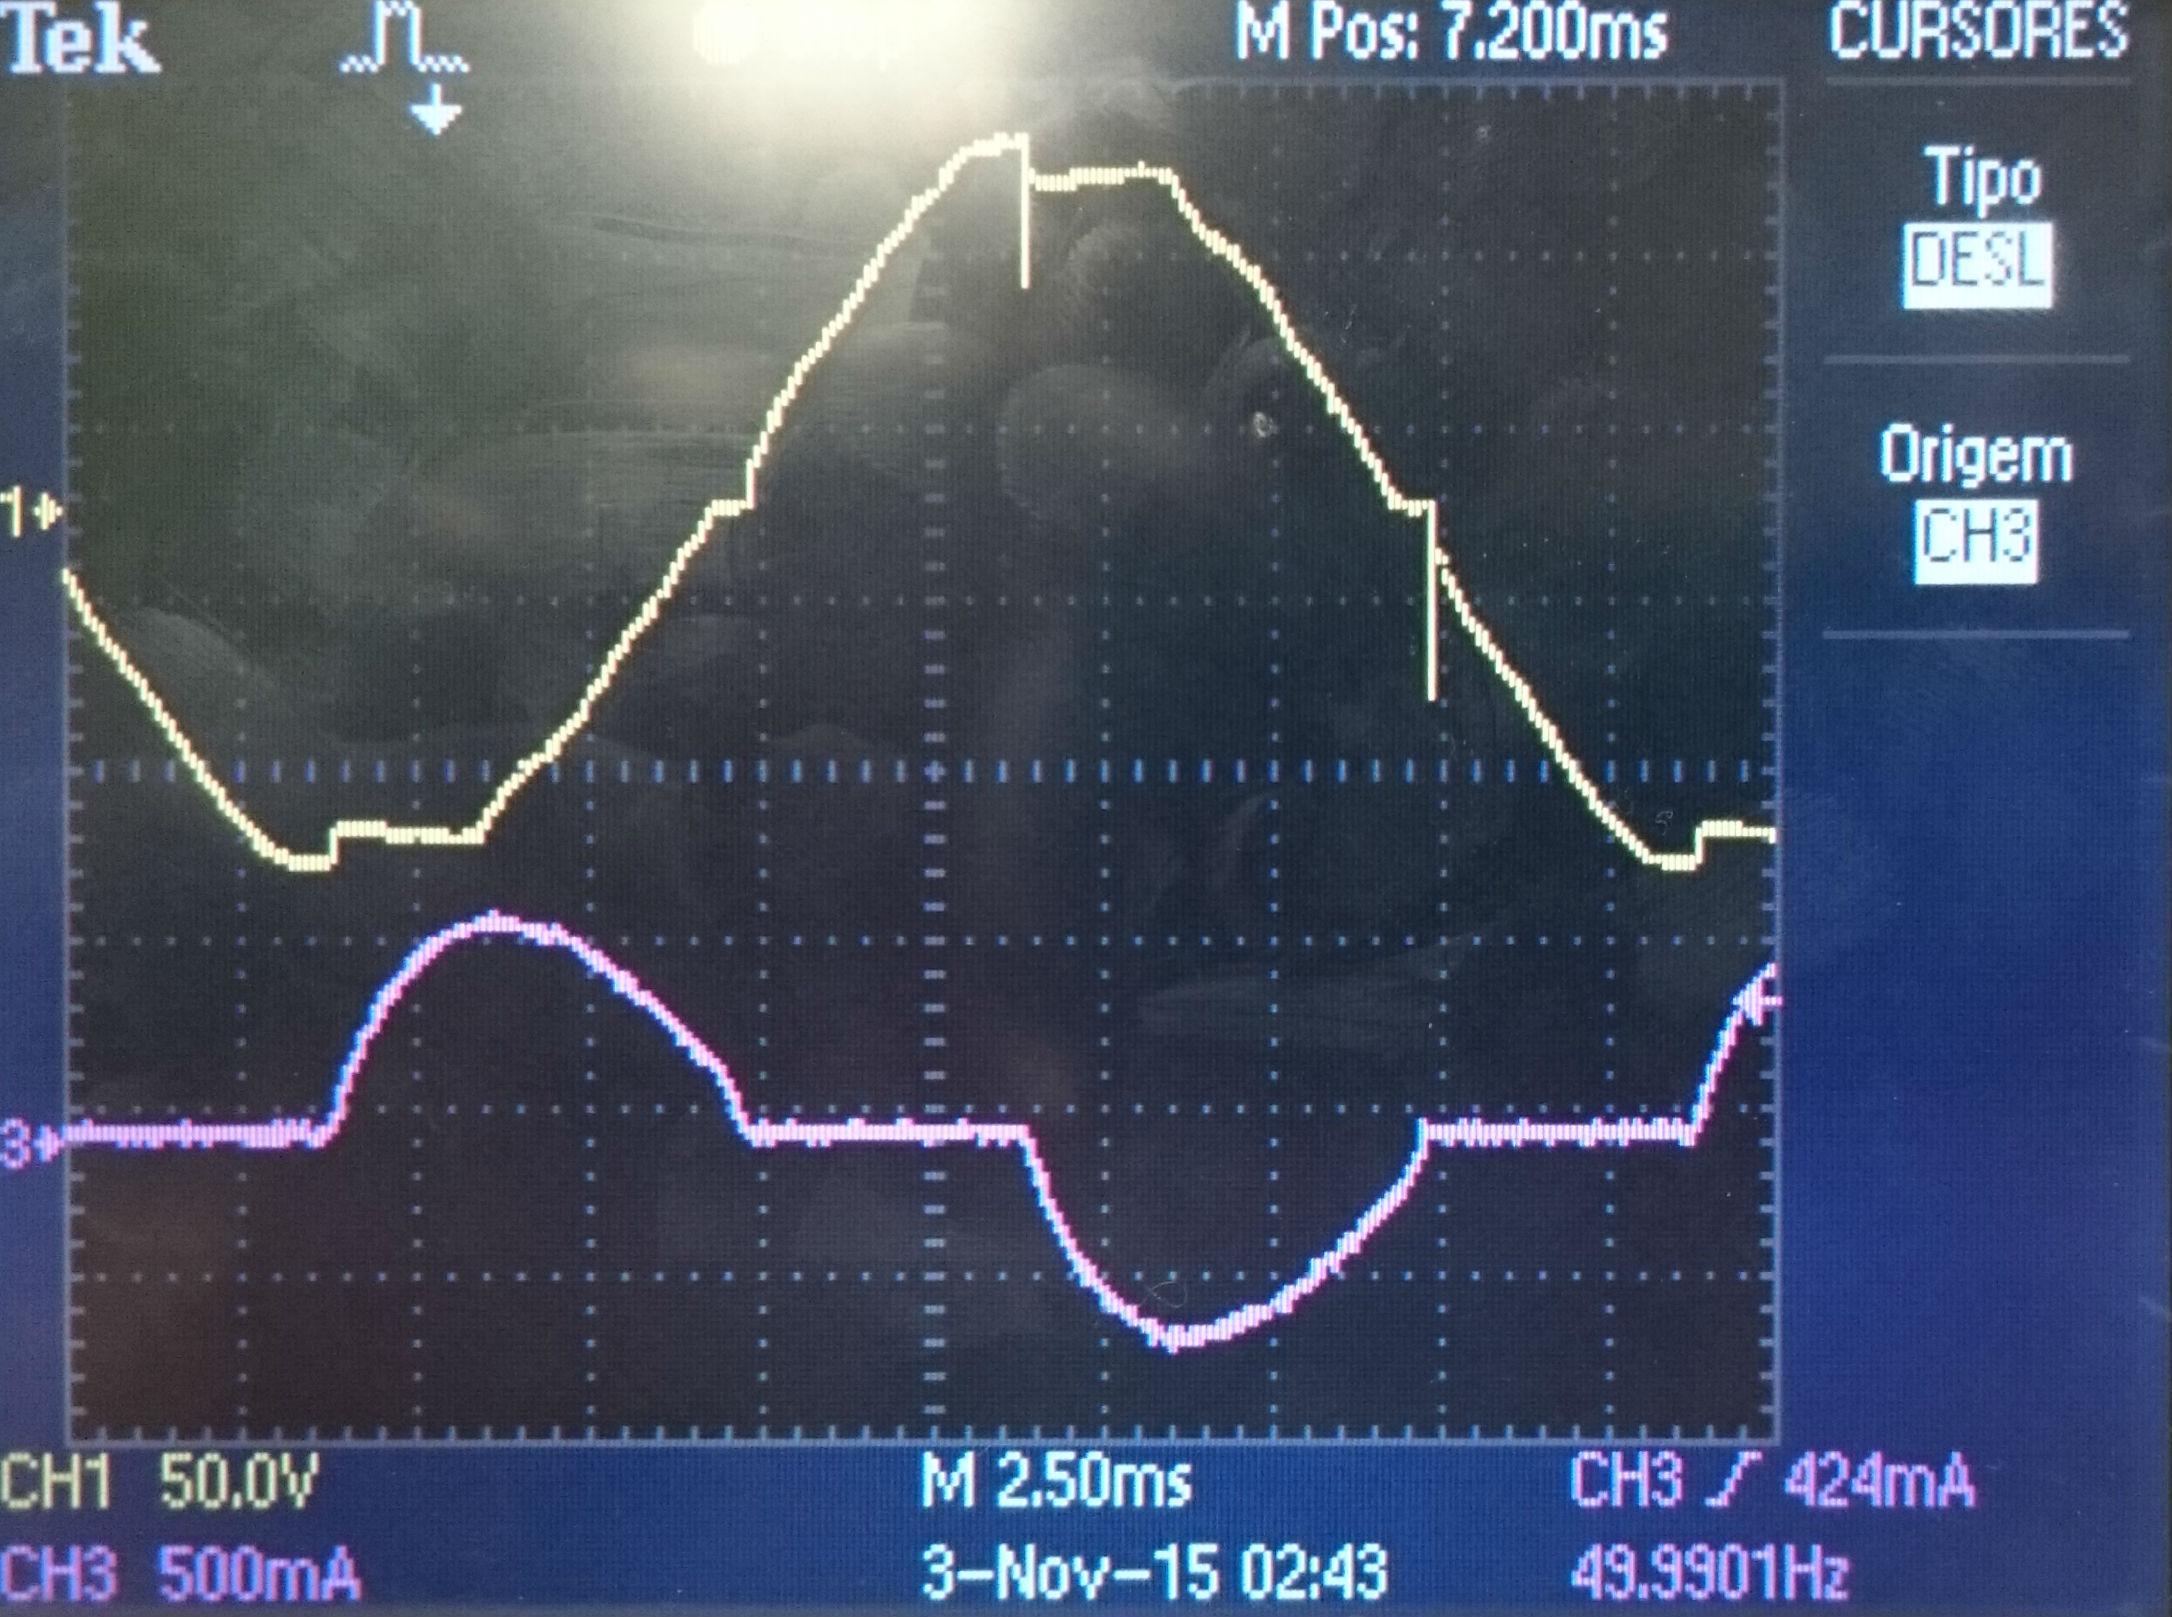
\includegraphics[keepaspectratio=true, scale=0.12]{img/DSC_0190}
	\caption{Tensão (a amarelo) e corrente (a rosa) na entrada.}
	\label{fig:tcentradasemi}
	\vspace{-0.8em}
\end{figure}

\paragraph{Formas de onda da tensão e corrente na carga} \mbox{}\

\begin{figure}[H]
	\centering
	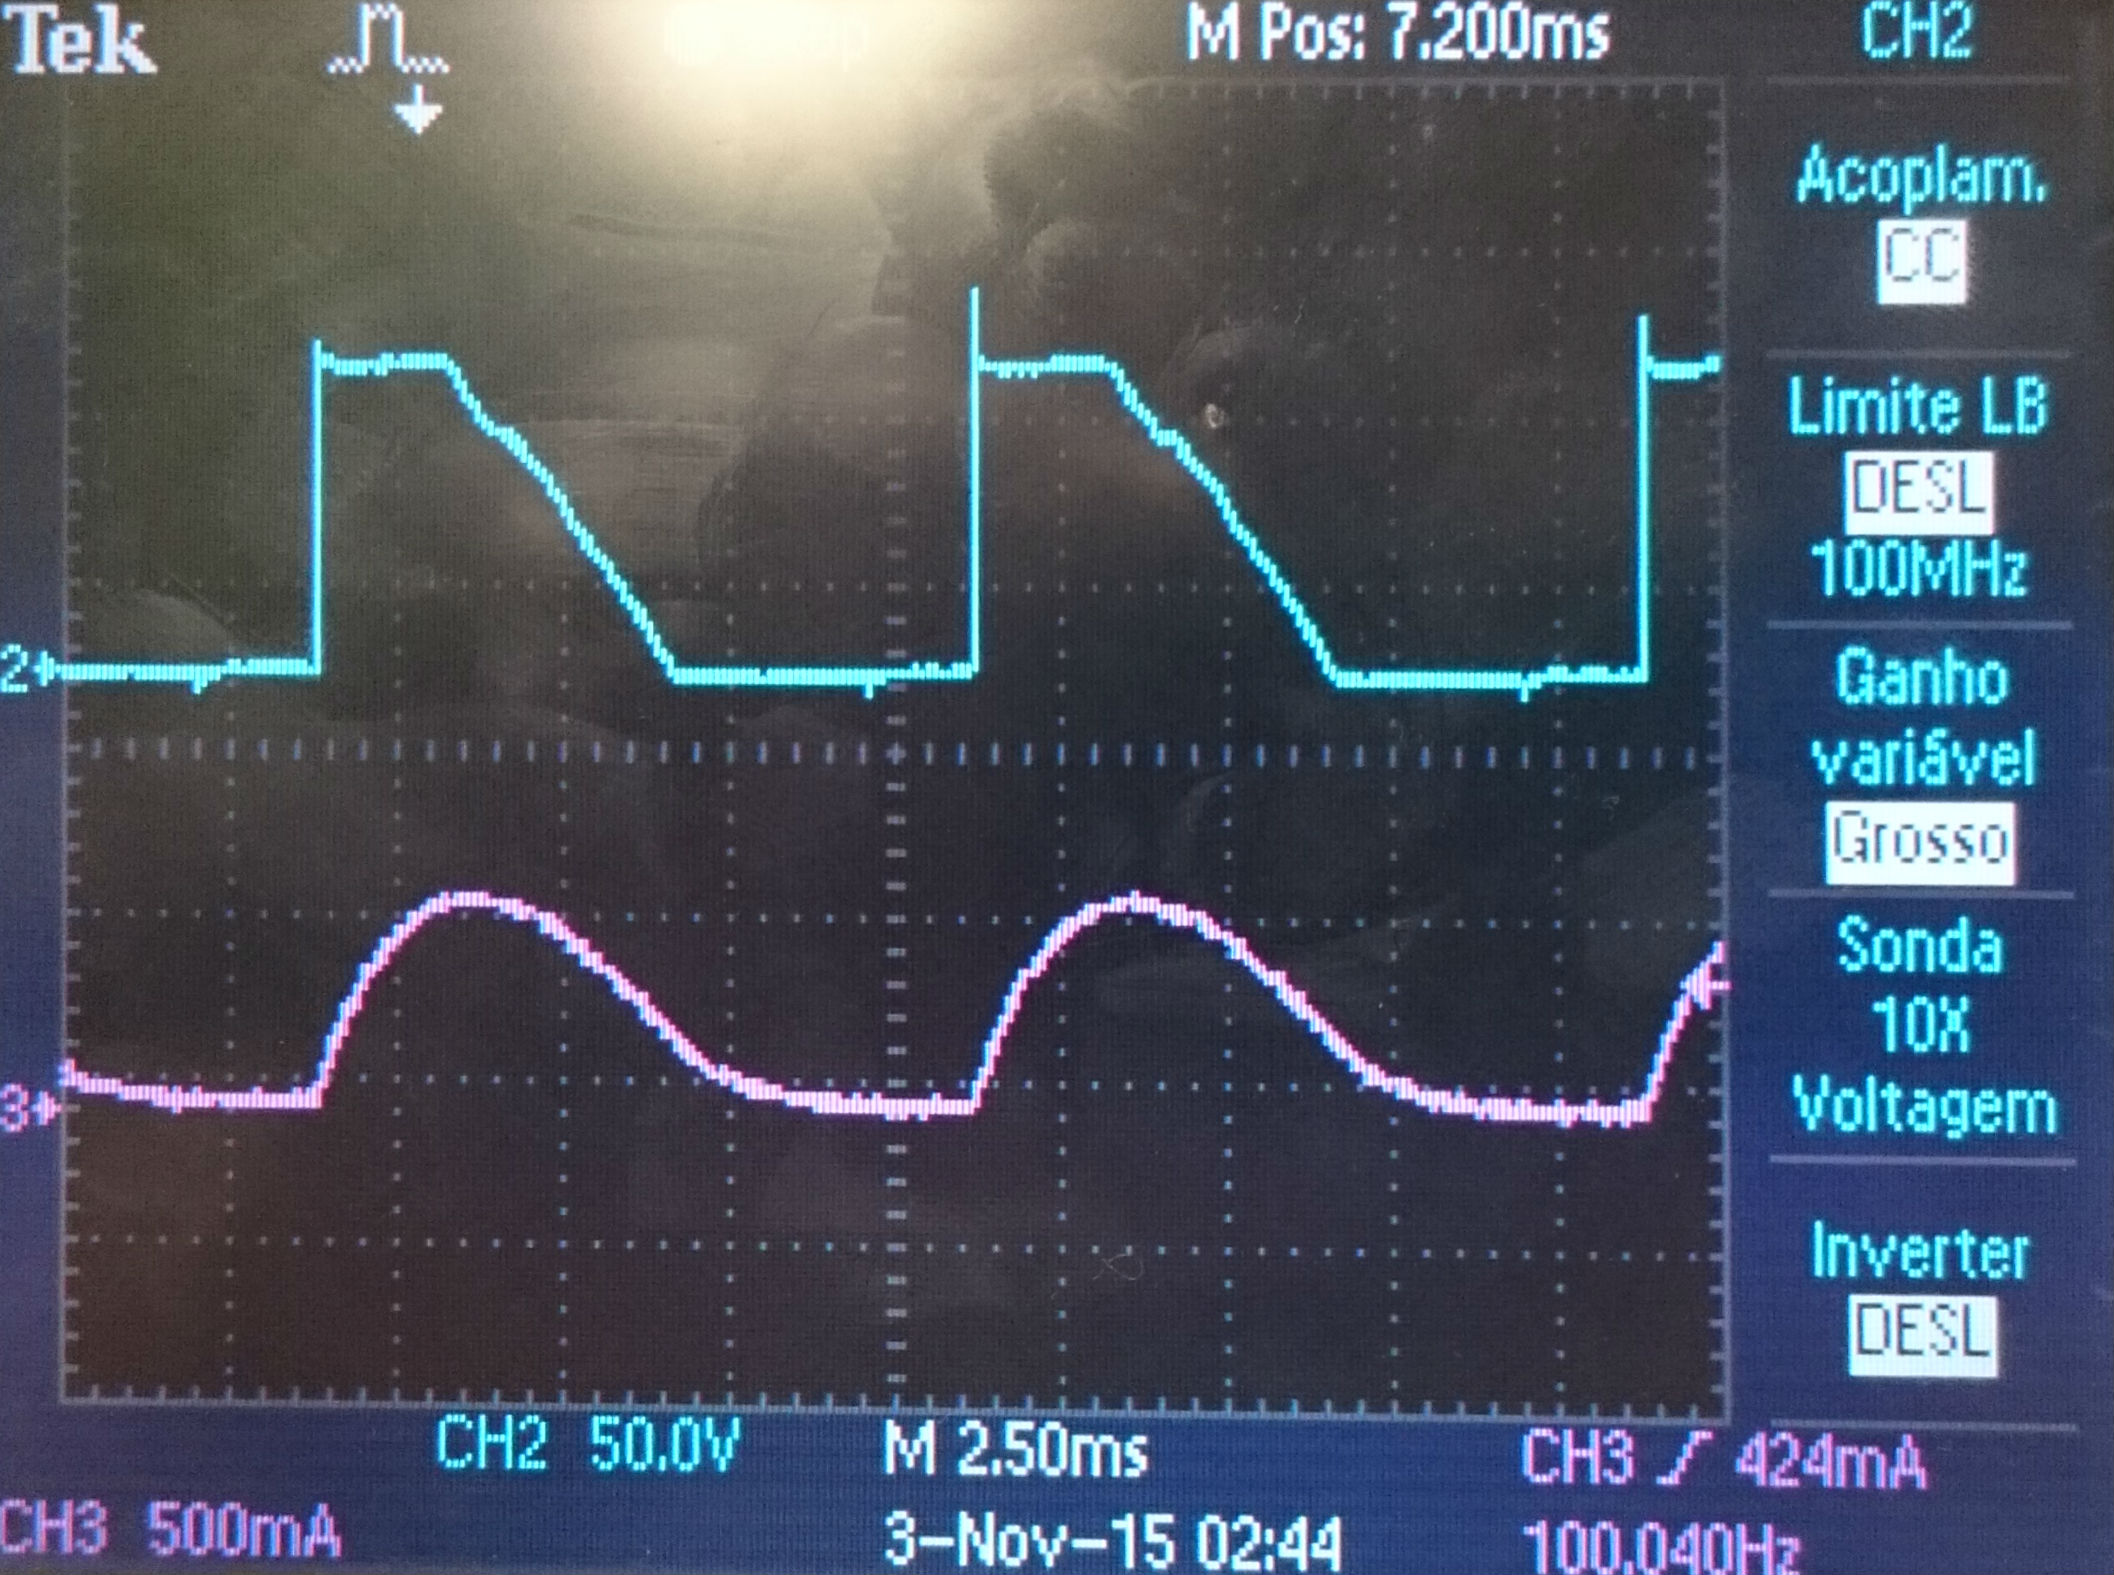
\includegraphics[keepaspectratio=true, scale=0.13]{img/DSC_0191}
	\caption{Tensão (a azul) e corrente (a rosa) na carga.}
	\label{fig:tccargasemi}
	\vspace{-0.8em}
\end{figure}

\paragraph{Formas de onda da tensão e corrente no tiristor} \mbox{}\

\begin{figure}[H]
	\centering
	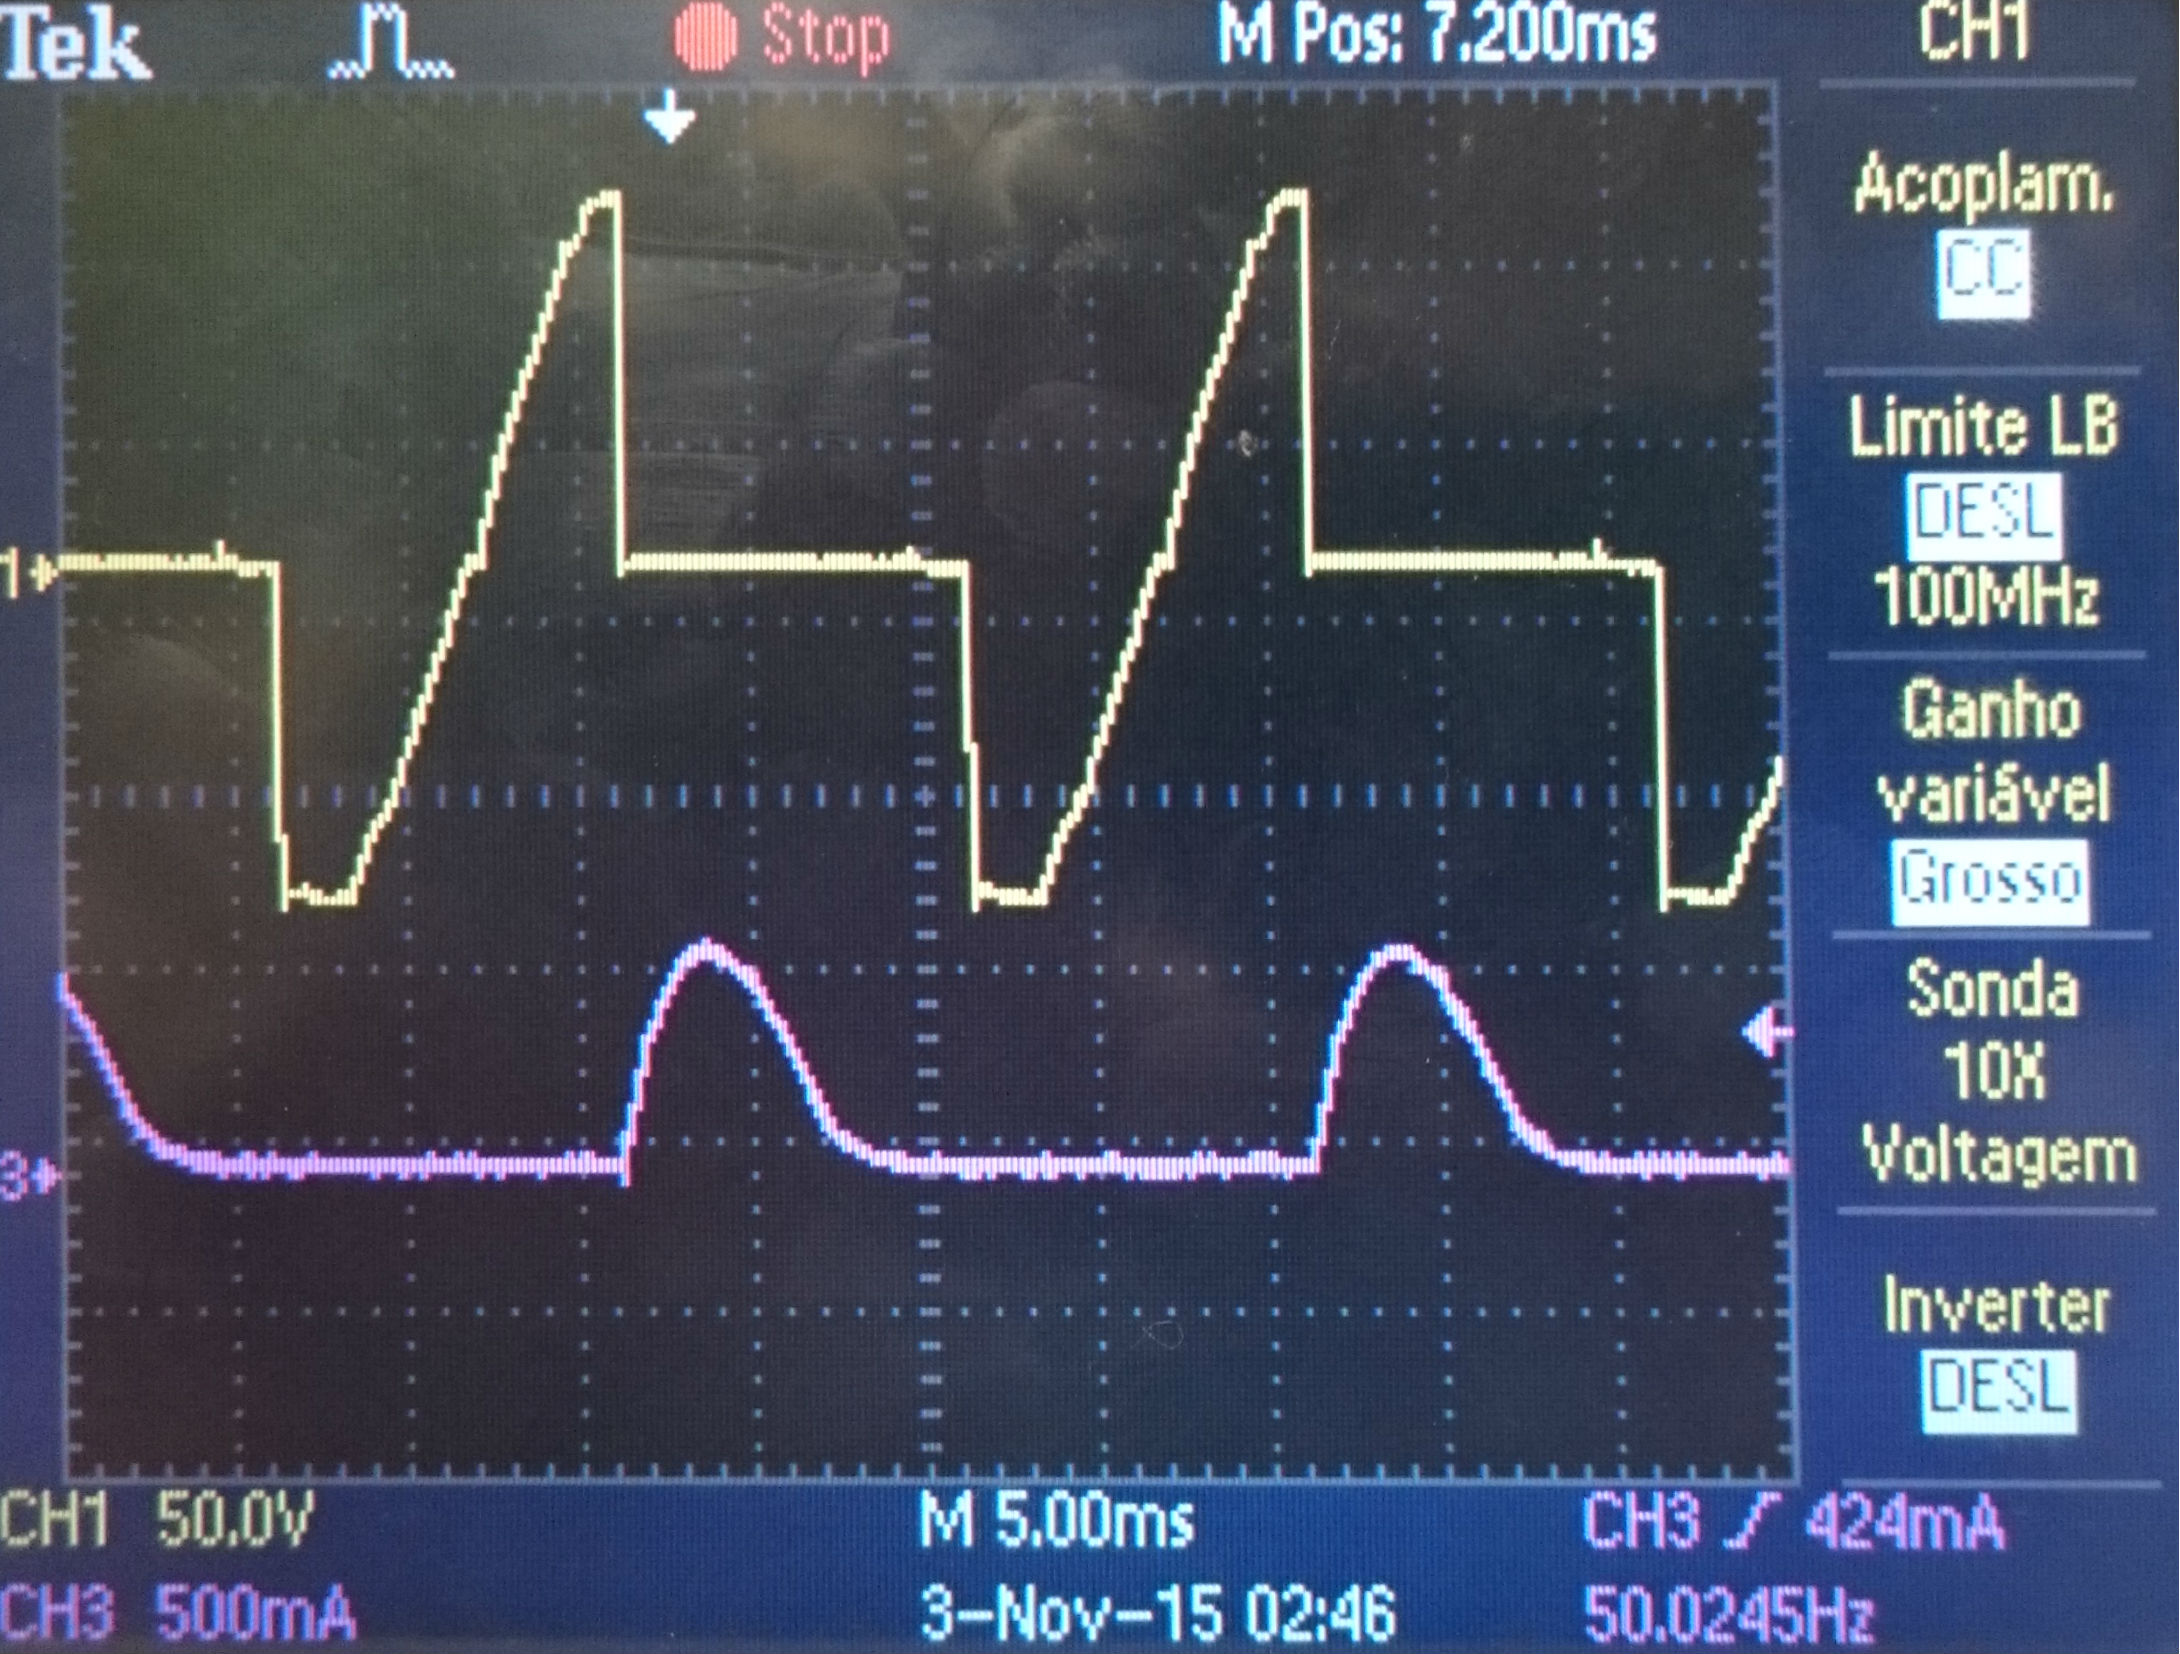
\includegraphics[keepaspectratio=true, scale=0.12]{img/DSC_0192}
	\caption{Tensão (a amarelo) e corrente (a rosa) no tiristor.}
	\label{fig:tctiristorsemi}
	\vspace{-0.8em}
\end{figure}

\paragraph{Característica de comando do conversor} \mbox{}\

\todo{porque razão a corrente na carga nunca é negativa}

\todo{valor médio da tensão na carga para ângulo de diaspor deo 60º}

\todo{dizer se é possivel utilizar este circuito para controlar a velocidade de um motor CC com travagem regenerativa}

\todo{que tipo de filtro utilizaria para exigências de conteúdo harmónico. Pode ligar-se um condensador em paralelo na saída do retificador? porque?}


\pagebreak

\begin{thebibliography}{2}
	
	%\bibitem{Kassakian}
	%Kassakian, John G. et al (1992, June), Principles of Power Electronics, \textit{Addison-Wesley Publishing Company}

	%\bibitem{Rashid}
	%Rashid, Muahammad H. (2004), Power Electronics - Circuits, Devices and Applications, \textit{Prentice Hall}
	
	\bibitem{Silva}
	Silva, Fernando (1998), Eletrónica Industrial, Fundação Calouste Gulbenkian
	
\end{thebibliography}


\pagebreak

\end{document}
